% ----------------------------------------------------------------------
\chapter{Grundlagen der Entwicklung der Benutzeroberflächen in Qt}
% ----------------------------------------------------------------------

\section{Was ist Qt? }
Qt ist ein quellfreies Framework und GUI-Toolkit zur plattformübergreifenden Entwicklung von Programmen und grafischen Benutzeroberflächen auf Grundlage der Programmiersprache C++ und für eine große Zahl an Betriebssystemen bzw. Grafikplattformen wie Linux, macOS, Windows, iOS und Android erhältlich.

\section {Kommunikation im Projekt}
Qt Creator ist eine integrierte Entwicklungsumgebung speziell für Qt und reduziert stark die Entwicklungsschwierigkeiten mit den Grundklassen, dem Qt Designer und die von Qt Creator am Anfang erstellten Codes wie Main Funktion, auf die im Folgenden näher eingegangen wird.   
\par Im Qt Creater stehen insgesamt 3 Grundklassen, nämlich QMainwindow, QWidget und QDialog, im ersten Schritt der Entwicklung zur Verfügung.  Q Mainwindow und QDialog sind abgeleitet von Q Widget. QWidget bietet einfach ein leeres Fenster. In QMainwindow  werden ein paar Leisten wie die Menüleiste, Statusleiste, die Symbolleiste, das Dock-Fenster und das mittlere leere Bereich automatisch erstellt. Und QDialog bietet ein Dialogfenster, um die Interaktion zwischen Benutzern und Programmen zu ermöglichen.
\par Mit Qt Designer wird das Fenster einfach konstruiert und erfolgreich aufgestellt, weil die gewünschten Menüeinträge einfach auf ein Fenster ziehen.  Und gleichzeitig werden die entsprechenden Codes sofort automatisch erstellt und aktualisiert.

\begin{figure}[h!]
	\centering
	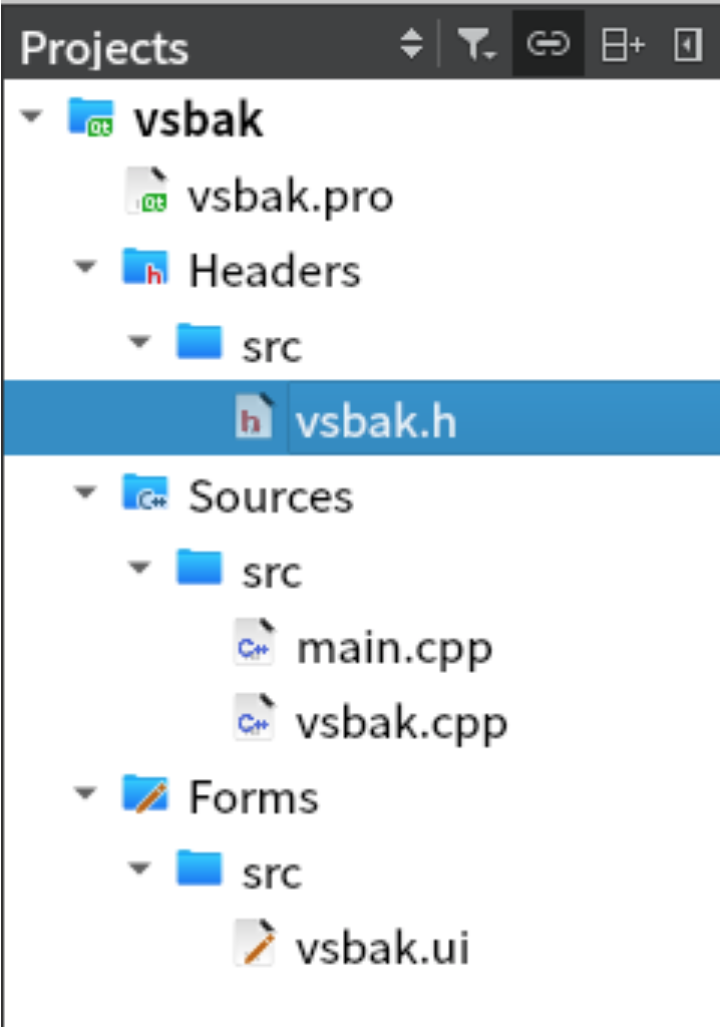
\includegraphics[width=0.4\textwidth]{bilder/verzeichnis.png}
	\caption{Verzeichnis des Projektes}
	\label{Abbildung_2}
\end{figure}

\par Am Beginn eines Projektes erzeugt Qt Creator automatisch 5 Dateien:eine Main-Datei, Pro-Datei, Header-Datei, Cpp-Datei und Ui-Datei. (s. Abbildung \ref{Abbildung_2}). 
\par In der Main Funktion sind zwei Objekte jeweils von der Klasse QApplication und einer der drei Grundklassen breit. Ausschließlich mit der Methode show() wird das Fenster gezeigt. 
\par Allerdings muss das Objekt der Klasse QAplication am Ende nach return noch die Methode exec() aufrufen. Die Methode dient dem stetigen Empfang der Nachrichten vom Benutzer.  
\par Pro-Datei beinhaltet die relevanten Informationen, wie zum Beispiel die Version der Entwicklungsumgebung, die benutzten Module, header Datei, Quellen Dateien u.s.w. Generell wird die Datei automatisch von IDE nach der gewünschten Konfiguration erstellt. Es ist erwähnenswert, dass die entsprechenden Orte von Cpp-Datei, Main-Datei,Header-Datei und Ui-Datei auch festgelegt werden.   
\par In Ui-Datei steht Qt Designer, nämlich ein grafisches Werkzeug zum Entwerfen und Erstellen der grafischen Benutzeroberflächen, zur Verfügung.   

